\documentclass{beamer-control}
\usepackage{beamer-control-singlefile}
\INCLUDEONLY{Basic Control Functions}
\begin{document}
\CONCEPT{Basic Control Functions}

\begin{SUMMARY}
\begin{itemize}
\item PID controller structure
\item P, I and D
\end{itemize}
\vfill References:
\begin{itemize}
\item \astrom{§11.1}
\end{itemize}
\end{SUMMARY}



\SUBCONCEPT{PID controller structure}

\begin{frame}{Control without a model}
\begin{itemize}
\item The PID controller is composed of three terms -- the proportional term (P) which depends on the present error, the integral term (I) which depends on the past error, and the derivative term (D) which depends on the future errors
\item Rather using a full state feedback controller based on a prediction of the future state of a system using a mathematical model, the PID controller uses linear extrapolation of the measured output for control
\item PID controllers are ubiquitous in industrial applications due to their wide applicability, ease of implementation, and avoidance of using a model
\end{itemize}
\end{frame}

\begin{frame}
\begin{figure}
	\centering
	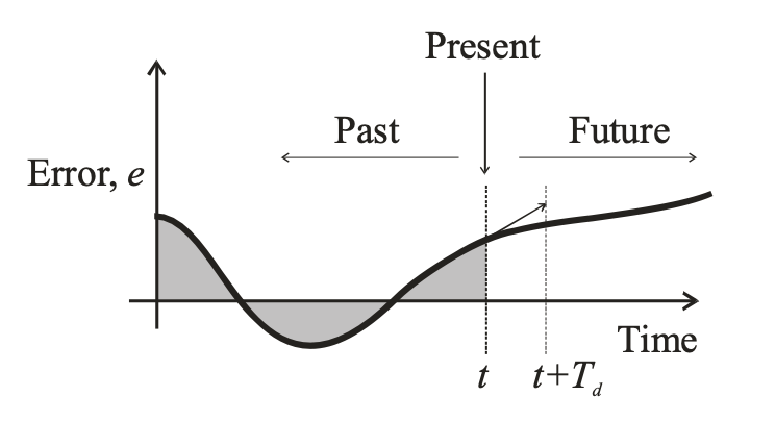
\includegraphics[width=0.8\linewidth]{figurePID1}
	\\
	\textbf{Figure:} Diagram describing the role of the three PID terms. 
\end{figure}
\end{frame}

\begin{frame}{Control action}
\begin{itemize}
	\item The control action of a PID controller is dependent on proportional feedback, integral action, and derivative action
	\[u=k_{p} e+k_{i} \int_0^t e(\tau) \, \mathrm{d} \tau+k_{d} \frac{\mathrm{d} e}{\mathrm{d} t}\]
	where $k_p$ is the proportional gain, $k_i$ is the integral gain, and $k_d$ is the derivative gain
	\item The integral time constant $T_i=\tfrac{k_p}{k_i}$ and derivative time constant $T_d = \tfrac{k_d}{k_p}$ provide an alternate parameterisation for the control action
	\[u = k_{p}\left(e+\frac{1}{T_{i}} \int_0^t e(\tau) \, \mathrm{d} \tau+T_{d} \frac{\mathrm{d} e}{\mathrm{d} t}\right)\]
\end{itemize}

\end{frame}


\begin{frame}
\begin{figure}
	\centering
	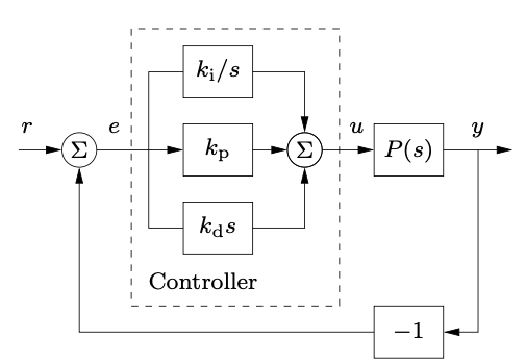
\includegraphics[width=0.8\linewidth]{figure11.1a}
	\\
	\textbf{Figure 11.1 (a):} Block diagram of PID controller in closed loop system. 
\end{figure}
\end{frame}

\SUBCONCEPT{P, I and D}

\begin{frame}{Effects of the three terms}{Proportional feedback}
\begin{itemize}
\item With only proportional feedback, non-zero steady-state error is common
\item Increasing the proportional gain $k_p$ will reduce the error but make the system more oscillatory
\item Too high of a gain may make the system unstable 
\item Proportional band also used, $PB=\tfrac{100}{k_p}$
\end{itemize}
\end{frame}

\begin{frame}{Effects of the three terms}{Integral feedback}
\begin{itemize}
	\item We saw in the Topic 4 - State Feedback that integral action guarantees that if a steady state exists, we will reach it with integral control
	\item An increase in the integral gain $k_i$ makes the system robust to disturbances
	\item Too high of a gain results in oscillatory behaviour, poor robustness, and possible instability
\end{itemize}
\end{frame}


\begin{frame}{Effects of the three terms}{Derivative feedback}
	\begin{itemize}
		\item Derivative control provides predictive or anticipatory action
		\item An increase in the derivative gain $k_d$ adds damping into the system
		\item Reduces overshoot
	\end{itemize}
\end{frame}

\begin{frame}{PID control implemented}
\begin{figure}
	\centering
	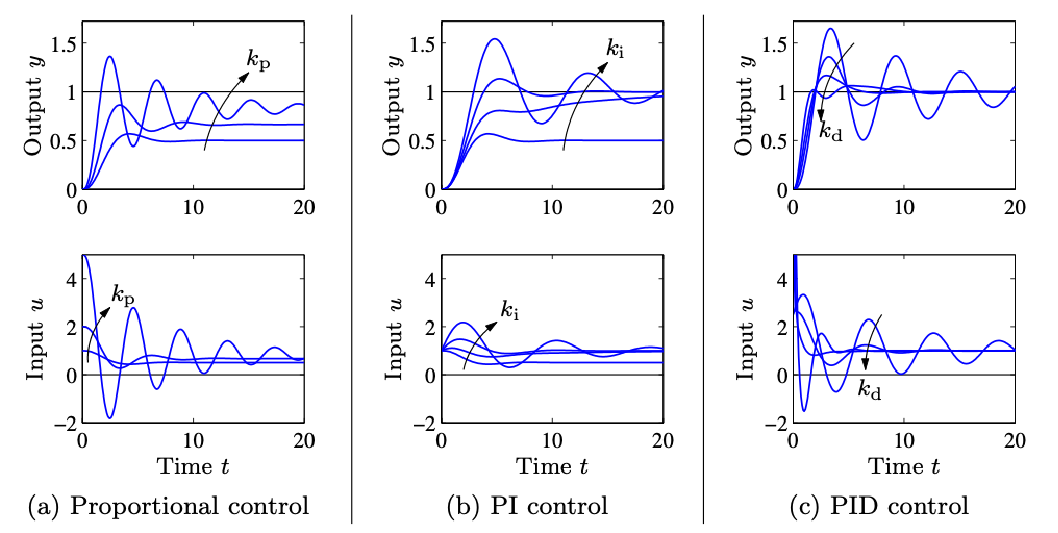
\includegraphics[width=\linewidth]{figure11.2}
	\\
	\textbf{Figure 11.2:} Responses to step changes in the reference value for a system with a proportional controller (a), PI controller (b), and PID controller (c).
\end{figure}
\end{frame}


\SUMMARYFRAME
\FINALE

\end{document}
